\documentclass[11pt]{article}

\usepackage{graphicx}

\title{Decoupled Software Pipelining in LLVM \\
        {\large 15-745 Final Project}}
\author{Fuyao Zhao and Mark Hahnenberg}
\date{}

\begin{document}

\maketitle

\section{Introduction}
\subsection{Problem}
Decoupled software pipelining presents an easy way to automatically extract thread-level parallelism for general loops in any program.  The compiler does this by examining the dependences of the loops in a given program, splitting the instructions of those loops into multiple smaller loops that execute in independent threads, and inserting dependence communication where necessary between these threads so that they remain synchronized.  The full process is described below in detail.  

\subsection{Approach}
We chose to implement DSWP using the general-purpose POSIX threading library (pthreads) and the Low Level Virtual Machine (LLVM) compiler infrastructure.  

\subsection{Related Work}
While DSWP has been implemented before, it was in the context of the IMPACT research compiler using customized hardware-level support on the Itanium platform.

\subsection{Contribution}
The decision to use LLVM will allow our implementation to be viewed in a context that is more relevant and more widely used than the IMPACT compiler, as LLVM is becoming not only a research but industry standard.  Due to our choice to use pthreads, Our DSWP implementation will also be portable across more platforms than previous implementations since any system that supports both LLVM and POSIX will be able to use our implementation, while former systems were limited to the Itanium platform with customized hardware support.

\section{Design}
\subsection{The Steps of DSWP}
DSWP can be described as a series of steps that first accumulate information about the program, then use that information to the extract the TLP from the program's loops, and finally modifies the program to execute in parallel those portions deemed to be parallelizable.

\subsubsection{Build Program Dependence Graph (PDG)}
In order to correctly insert dependence flows among the independently running sub-loops that are generated we need to enumerate the various dependences among the instructions in each loop within the program.  These dependences can be classified into two categories: data dependences and control dependences.  We build the PDG containing this information as our first step as in Figure~\ref{pdg}.

This process is different than how it was described in the paper.  The paper used a method of peeling off the first iteration of the loop and running normal dependence analysis on that graph and then coalescing the duplicated nodes afterward to fit the original graph.  This was difficult in LLVM because of the fact that LLVM is in SSA form, so it would have been unclear as to how to modify the program graph to make this work.

\begin{figure}
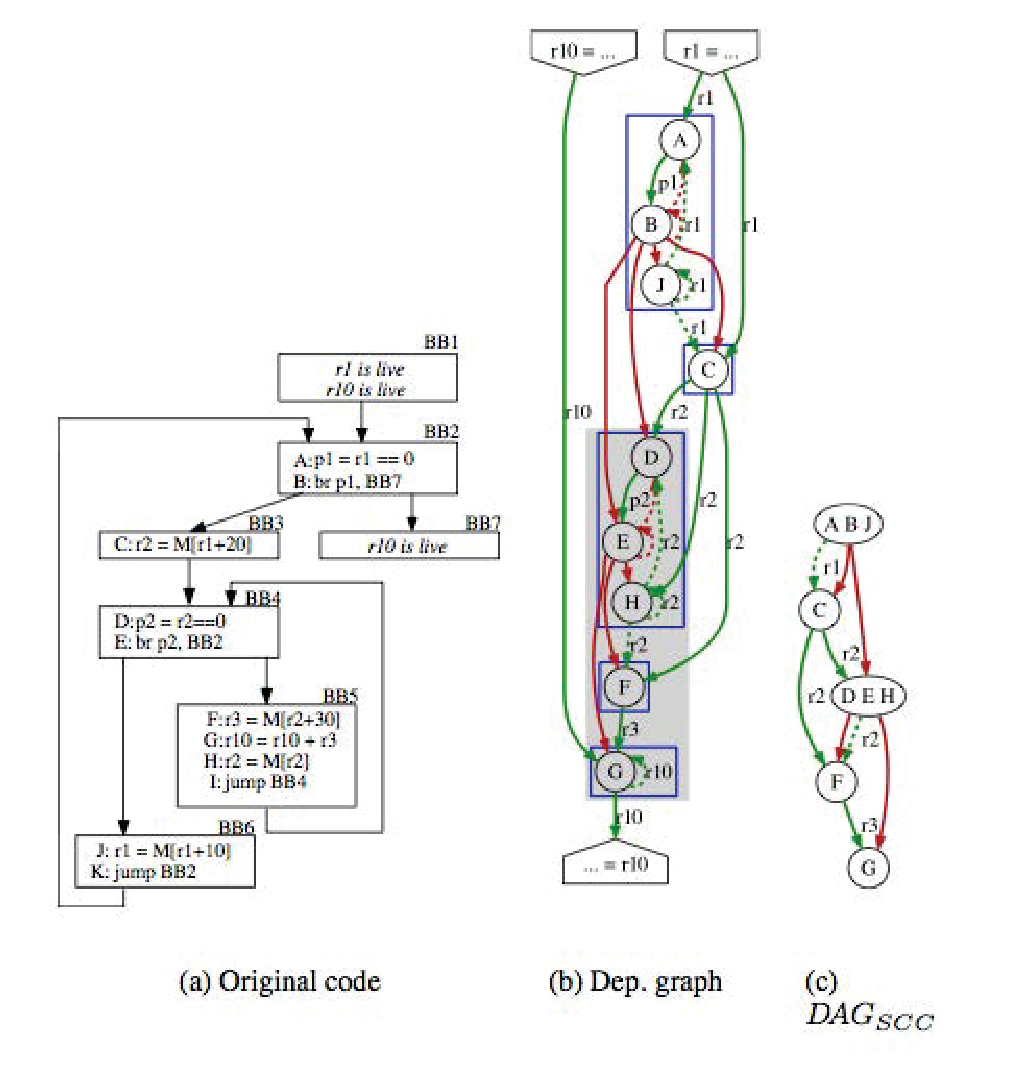
\includegraphics[scale=0.75]{pdg}
\caption{Illustrates the original program (a), the PDG based on that code (b), and the $DAG_{SCC}$ generated using the PDG.}
\label{pdg}
\end{figure}

\subsubsection{Find Strongly Connected Components (SCC) and Coalesce into a DAG}
In the next step, we take the PDG and find the strongly connected components in it.  We do this to ensure that there are no cycles in the resulting graph when we coalesce the nodes, which is necessary to form a pipeline.  Each of these SCCs represents cyclic dependences within the loop, so the compiler requires that these remain in the same thread.  After we have found the SCCs, we coalesce each of them into single nodes to form a DAG.  Refer to Figure~\ref{pdg} for an illustration of this process.

\subsubsection{Assign Partitions of DAG to Threads}
Our goal for the next step is to partition the nodes of the DAG among a fixed set of threads.  A valid partitioning $P$ is such that all of the dependence arcs either are within the same $P_i \in P$ or they go from $P_i$ to $P_j$ such that $i < j$, thus forming a pipeline between the partitions.  We want to choose a partitioning among the threads such that we minimize our overall execution time.  While this general problem is NP-complete, we use the heuristic from the paper to provide an estimation for a given partition of the DAG.

\subsubsection{Split Partitions into Loops}
After we find a valid partitioning of the nodes, we create a new function for each partition and copy in the relevant instructions for those partitions.  In the original thread, we send the addresses of these functions to the waiting threads.

\subsubsection{Insert Dependence Synchronization}
After generating the new functions to be assigned to the separate threads, we need to insert the dependence communication between the partitions.  We need some additional control dependences that aren't captured by traditional control dependences.  Since different synchronization queues can be used on consecutive iterations, we must synchronized the threads iteration by iteration.  Essentially we need the header to have a control dependence on any block that branches either to the exit or to the header.  We do this simply by checking each branch instruction within the loop to see if it goes back to the loop header.  If it does, then we mark the header as depending on that block.  See Figure~\ref{sync} for an example of code being split across two threads and the resulting produce and consume sites that must be inserted.

\begin{figure}
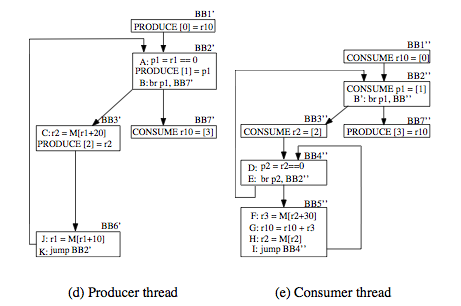
\includegraphics[scale=0.75]{sync}
\caption{Illustrates the splitting of code across threads and the insertion of synchronization primitives (produce (d) and consume (e)).}
\label{sync}
\end{figure}

\subsubsection{Runtime Support}
The compiler needs the support of a runtime library that will manipulate the necessary synchronization primitives.  A separate synchronization library (simple\_sync.c) is linked with the regular source code at compile time.  This library, in turn, uses queue.c as its queue implementation.  We statically create 256 dependence queues.  Each queue has length 32.  If the queue is empty, pop operations will block until a value is pushed into the queue.  If the queue is full, push operations will block until space becomes available.  The locations where produce and consume instructions are inserted into the program during compilation are simply function calls to this library.

At the beginning of each loop the new threads are created and sent the address of the function they are to execute.  Each dependence gets its own queue. We statically create 256 queues to use for the various dependences.  Each produce in the thread that generates the dependence is matched by a single consume in the thread that requires that dependence.

\section{Experimental Setup}
We built a loadable module for LLVM that can be called as a separate optimization pass.  We then ran this pass on the otherwise unoptimized SPEC2006 benchmarks.  We compared these results with the results of running the completely unoptimized SPEC2000 benchmarks.

\section{Experimental Results}


\section{Lessons Learned}
Academic papers are not always explicit about the steps they take in their implementations.  We had to intuit many of the necessary details to make the compilation process work.

\section{Conclusions}


\end{document}
